%%%%%%%%%%%%%%%%%%%%%%%%%%%%%%%%%%%%%%%%%%%%%%%%%%%%%%%%%%%%%%%%%%%%%%%%%%%%%%%%%%%%
% Document data
%%%%%%%%%%%%%%%%%%%%%%%%%%%%%%%%%%%%%%%%%%%%%%%%%%%%%%%%%%%%%%%%%%%%%%%%%%%%%%%%%%%%
\documentclass[12pt]{article} %report allows for chapters
%%%%%%%%%%%%%%%%%%%%%%%%%%%%%%%%%%%%%%%%%%%%%%%%%%%%%%%%%%%%%%%%%%%%%%%%%%%%%%%%%%%%
\usepackage{preamble}

\begin{document}

\begin{center}
   \textsc{\large MATH 272, Homework 6, \emph{Solutions}}\\
   \textsc{Due March \textcolor{red}{24}$^\textrm{th}$}
\end{center}
\vspace{.5cm}


\begin{problem} 
Let 
\[
\curvegamma(t) = \begin{pmatrix} \cos(t) \\ \sin(t) \\ t \end{pmatrix}, \quad f(x,y,z) = x^2 + y^2 - 2z^2, \quad \vecfieldV(x,y,z) = \begin{pmatrix} x-y \\ y+x \\ z \end{pmatrix}.
\]
Compute derivatives of the following composite functions.
\begin{enumerate}[(a)]
	\item $f(\curvegamma(t))$.
	\item $\vecfieldV(\curvegamma(t))$.
	\item $f(\vecfieldV(x,y,z))$.
\end{enumerate}
\end{problem}
\begin{solution}~
    \begin{enumerate}[(a)]
        \item   We are considering the composite function $f\circ \curvegamma \colon \R \to \R$.  Hence, our result for the derivative must be a linear function $(f\circ \curvegamma)' \colon \R \to \R$.  Specifically, this means that at any time $t$, we have a $1\times 1$-matrix as the derivative. Following our nose, we can use the chain rule
        \[
        (f\circ \curvegamma)' = \grad f(\curvegamma(t))\tangentgamma(t).
        \]
        Note that here we think of $\grad f$ as the $1\times 3$ \emph{row} vector (which is often called a covector).  Why is that? Well, recall that $f\colon \R^3 \to \R$ and hence the derivative is a linear function $f' = \grad f \colon \R^3 \to \R$.  Hence, $\grad f$ must be a matrix that multiplies by a column vector (a $3\times 1$-matrix) and gives us a number.  This must mean that $\grad f$ is a $1\times 3$-matrix.  Now,
        \[
        \grad f = \begin{pmatrix} 2x & 2y & -4z \end{pmatrix},
        \]
        and
        \[
        \grad f(\curvegamma(t)) = \begin{pmatrix} 2\cos(t) & 2\sin(t) & -4t \end{pmatrix}.
        \]
        Then,
        \[
        \tangentgamma(t) = \begin{pmatrix} -\sin(t) \\ \cos(t) \\ 1 \end{pmatrix}.
        \]
        Thus,
        \begin{align*}
        \grad f(\curvegamma(t))\tangentgamma(t) &= \begin{pmatrix} 2\cos(t) & 2\sin(t) & -4t \end{pmatrix}\begin{pmatrix} -\sin(t) \\ \cos(t) \\ 1 \end{pmatrix}\\
        &= -2\cos(t)\sin(t) + 2\cos(t)\sin(t) -4t\\
        &=-4t.
        \end{align*}
        
        \item Now $\vecfieldV \circ \curvegamma \colon \R \to \R^3$ and so we are expecting a $3\times 1$-matrix result.  In this case, it will be given by
        \[
        \left( \vecfieldV \circ \curvegamma\right)' = [J]_{\vecfieldV}(\curvegamma(t))\tangentgamma(t).
        \]
        We compute the derivative of $\vecfieldV$ as the Jacobian
        \[
        [J]_{\vecfieldV}(x,y,z) = \begin{pmatrix} 1 & -1 & 0 \\ 1 & 1 & 0 \\ 0 & 0 & 1 \end{pmatrix},
        \]
        which is constant. This means that
        \[
        [J]_{\vecfieldV}(\curvegamma(t)) = \begin{pmatrix} 1 & -1 & 0 \\ 1 & 1 & 0 \\ 0 & 0 & 1 \end{pmatrix}.
        \]
        We already computed $\tangentgamma$, and thus
        \begin{align*}
        [J]_{\vecfieldV}(\curvegamma(t))\tangentgamma(t) &= \begin{pmatrix} 1 & -1 & 0 \\ 1 & 1 & 0 \\ 0 & 0 & 1 \end{pmatrix}\begin{pmatrix} -\sin(t) \\ \cos(t) \\ 1 \end{pmatrix} \\
        &= \begin{pmatrix} -\sin(t)-\cos(t) \\ -\sin(t) +\cos(t) \\ 1 \end{pmatrix}.
        \end{align*}
        
        \item Finally, note $f\circ \vecfieldV \colon \R^3 \to \R$, which means we expect a $1\times 3$ matrix for $(f\circ \vecfieldV)'$.  We have that
        \[
        (f\circ \vecfieldV)' = \grad f(\vecfieldV(x,y,z)) [J]_{\vecfieldV}(x,y,z),
        \]
        where again we think of $\grad f$ as a covector.  Now, this yields
        \begin{align*}
        \grad f(\vecfieldV(x,y,z)) [J]_{\vecfieldV}(x,y,z) &= \begin{pmatrix} 2(x-y) & 2(x+y) & -4z \end{pmatrix} \begin{pmatrix} 1 & -1 & 0 \\ 1 & 1 & 0 \\ 0 & 0 & 1 \end{pmatrix}\\
        &= \begin{pmatrix} 4x & 4y & -4z \end{pmatrix}.
        \end{align*}
    \end{enumerate}
    
\end{solution}

\newpage
\begin{problem}
Show that for any smooth (more than twice differentiable) fields $f(x,y,z)$ and $\vecfieldV(x,y,z)$ that
\begin{enumerate}[(a)]
	\item $\grad \times \left(\grad f\right)=\boldsymbol{\vec{0}}$;
	\item $\grad \cdot \left(\grad \times \vecfieldV\right)=0$.
\end{enumerate}
\end{problem}
\begin{solution}~
    \begin{enumerate}[(a)]
        \item We have that 
        \[
        \grad f = \begin{pmatrix} \frac{\partial f}{\partial x} \\ \frac{\partial f}{\partial y} \\ \frac{\partial f}{\partial z}\end{pmatrix} = \begin{pmatrix} V_1 \\ V_2 \\ V_3 \end{pmatrix}.
        \]
        Taking the curl yields
        \[
        \grad \times \left(\grad f\right) = \begin{pmatrix} \frac{\partial V_3}{\partial y} - \frac{\partial V_2}{\partial z} \\ \frac{\partial V_1}{\partial z} - \frac{\partial V_3}{\partial x} \\ \frac{\partial V_2}{\partial x} - \frac{\partial V_1}{\partial y} \end{pmatrix} = 
        \begin{pmatrix} \frac{\partial^2 f}{\partial z\partial y} - \frac{\partial^2 f}{\partial y\partial z} \\ \frac{\partial^2 f}{\partial x\partial z} - \frac{\partial^2 f}{\partial z \partial x} \\ \frac{\partial^2 f}{\partial y\partial x} - \frac{\partial f}{\partial x\partial y} \end{pmatrix}= \begin{pmatrix} 0 \\ 0 \\ 0 \end{pmatrix},
        \]
        since partial derivatives commute for any smooth scalar field.
        
        \item First, the curl is
        \[
        \grad \times \vecfieldV = \begin{pmatrix} \frac{\partial V_3}{\partial y} - \frac{\partial V_2}{\partial z} \\ \frac{\partial V_1}{\partial z} - \frac{\partial V_3}{\partial x} \\ \frac{\partial V_2}{\partial x} - \frac{\partial V_1}{\partial y} \end{pmatrix},
        \]
        and we can take the divergence
        \begin{align*}
            \grad \cdot \left(\grad \times \vecfieldV\right) &= \frac{\partial}{\partial x} \left(\frac{\partial V_3}{\partial y} - \frac{\partial V_2}{\partial z}\right) +  \frac{\partial}{\partial y} \left(\frac{\partial V_1}{\partial z} - \frac{\partial V_3}{\partial x}\right) +  \frac{\partial}{\partial z} \left(\frac{\partial V_2}{\partial x} - \frac{\partial V_1}{\partial y}\right)\\
            &= 0,
        \end{align*}
        again since partial derivatives commute.
    \end{enumerate}
\end{solution}

\newpage
\begin{problem}
	Let 
	\[
	\vecfieldU(x,y,z) = \begin{pmatrix} -y \\ x \\ 0 \end{pmatrix} \qquad \textrm{and} \qquad \vecfieldV(x,y,z) = \begin{pmatrix} 2x \\ 2y \\ 2z \end{pmatrix},
	\] 
	be vector fields.  
	\begin{enumerate}[(a)]
		\item Explain why there exists no potential function $\phi(x,y,z)$ for the vector field $\vecfieldU$.
		\item Explain why there does exist a potential function $\phi(x,y,z)$ for the field $\vecfieldV$.
		\item Compute the potential function for $\vecfieldV$.
	\end{enumerate}
\end{problem}
\begin{solution}~
    \begin{enumerate}[(a)]
        \item There exists a potential function if the curl of $\vecfieldU$ is zero.  So, taking the curl we find
        \[
        \grad \times \vecfieldU = \begin{pmatrix} 0 \\ 0 \\ 2 \end{pmatrix},
        \]
        which is nonzero. Thus, there cannot be a potential function for $\vecfieldU$.
        
        \item Likewise, taking the curl for $\vecfieldV$ we get
        \[
            \grad\times \vecfieldU = \begin{pmatrix} 0 \\ 0 \\ 0 \end{pmatrix}.
        \]
        Hence, there must be a potential function for $\vecfieldV$.  
        
        \item To compute the potential $\phi(x,y,z)$, we integrate $V_1$ with respect to $x$, $V_2$ with respect to $y$, and $V_3$ with respect to $z$.  This yields
        \begin{align*}
            \phi(x,y,z) &= \int 2x dx = x^2+\psi_1(y,z)\\
            \phi(x,y,z) &= \int 2y dy = y^2+\psi_2(x,z)\\
            \phi(x,y,z) &= \int 2z dz = z^2+\psi_3(x,y).
        \end{align*}
        Since these are all equal, we must have that
        \[
        \phi(x,y,z) = x^2+y^2+z^2+C,
        \]
        where $C$ is a constant.
    \end{enumerate}
\end{solution}

\newpage
\begin{problem} 
Parameterize the following either implicitly or explicitly. In Cartesian coordinates, find the parameterization of the normal vector as well.
\begin{enumerate}[(a)]
	\item The plane perpendicular to the vector $\vecv = \xhat + \yhat + \zhat$ passing through the point $(1,1,1)$.
	\item The upper half of the unit circle in $\R^2$.
	\item The surface of the unit sphere in $\R^3$.
\end{enumerate}
\end{problem}
\begin{solution}~
    \begin{enumerate}[(a)]
        \item Based on the vector perpendicular to the plane $\vecv$, we are looking for a plane given by
        \[
        0=a(x-x_0)+b(y-y_0)+c(z-z_0),
        \]
        where we have
        \[
        \begin{pmatrix} a \\ b \\ c \end{pmatrix} = \begin{pmatrix} v_1 \\ v_2 \\ v_3 \end{pmatrix} = \begin{pmatrix} 1 \\ 1 \\ 1 \end{pmatrix}.
        \]
        Similarly, we wish to have the plane pass through the point $(1,1,1)$ hence
        \[
        (x_0,y_0,z_0)=(1,1,1).
        \]
        Thus, our implicit equation for this plane is
        \[
        0=(x-1)+(y-1)+(z-1).
        \]
        
        We could also give an explicit equation for the plane as the graph of a function.  Specifically, we have from the above work
        \[
        z=-x-y+3.
        \]
        Thus, as a graph we would take the plane to be given by the points
        \[
        (x,y,-x-y+3).
        \]
        One could also find two linearly independent vectors perpendicular to $\vecv$ and based at $(1,1,1)$ and take their span.
        
        \item Implicitly, the unit circle is the set of all points a distance 1 from the origin.  Thus, we are looking for $(x,y)$ pairs that satisfy
        \[
        \sqrt{x^2+y^2}=1.
        \]
        Note that we could also write this as
        \[
        x^2+y^2=1.
        \]
        Then, to receive the upper semi circle, we simply neglect values of $y<0$ to get the implicit description
        \[
        x^2+y^2=1 \qquad \textrm{with $y\in [0,1]$.}
        \]
        
        Explicitly, we can solve for $y$ in terms of $x$ from the previous work to get
        \[
        y=\pm \sqrt{1-x^2}.
        \]
        Taking $y=\sqrt{1-x^2}$ we know $y\geq 0$, and this gives us the upper half of the unit circle as the graph of a function. 
        
        Or, we could parameterize this as a curve to get another implicit description.  We know the curve $\curvegamma(t) = \begin{pmatrix} \cos(t) \\ \sin(t)\end{pmatrix}$ lie on the unit circle for all times $t$.  Then, if we restrict $t\in [0,\pi]$, this gives us just the upper half.
        
        \item Similarly to (b), the surface of the unit sphere is the set of points a distance 1 from the origin and so we can write this as an implicit equation
        \[
        x^2+y^2+z^2=1.
        \]
        
        Explicitly, we could solve for $z$ from the above work to get two graphs
        \[
        z = \pm \sqrt{1-x^2-y^2},
        \]
        which if we combine, gives us an explicit description of the surface of the unit sphere.  
        
        One could also arrive at a different explicit description of the unit sphere by using spherical coordinates. Take $\phi$ to the angle from the $z$-axis of a point on the sphere and $\theta$ to be the polar angle from the $xz$-plane and we have that the points on the surface of the unit sphere are given by
        \[
        \begin{pmatrix} \cos\theta\sin\phi \\ \sin\theta \sin \phi \\ \cos \phi \end{pmatrix},
        \] 
        where $\theta \in [0,2\pi)$ and $\phi \in [-\pi,\pi]$.
    \end{enumerate}
\end{solution}

\newpage
\begin{problem}
	In cylindrical coordinates (either implicitly or explicitly), parameterize the following objects.
	\begin{enumerate}[(a)]
		\item A cylinder with radius 3 and height 5 along with end-caps.
		\item An infinite cone with a vertex angle of $\pi/4$.
		\item A helical curve with constant radius 1 and pitch 1.
		\item A hyperboloid of one sheet.
	\end{enumerate}
\end{problem}
\begin{solution} We will find the natural paramaterizations of these shapes are natural (and thus explicit) in these coordinates.
    \begin{enumerate}[(a)]
        \item If we have a cylinder of radius 3, then we have that $\rho=3$.  If the height is $5$, we can just take $z\in [0,5]$.  The end caps can be described by the points satisfying $\rho<3$ and $z=0$ for the bottom cap as well as $\rho<3$ and $z=5$ for the top cap. This is an explicit description.
        \item Here, we can take the look at a cone from a side profile and notice that we get $\rho=Cz$ where $C$ is a constant.  
        \begin{figure}[H]
            \centering
            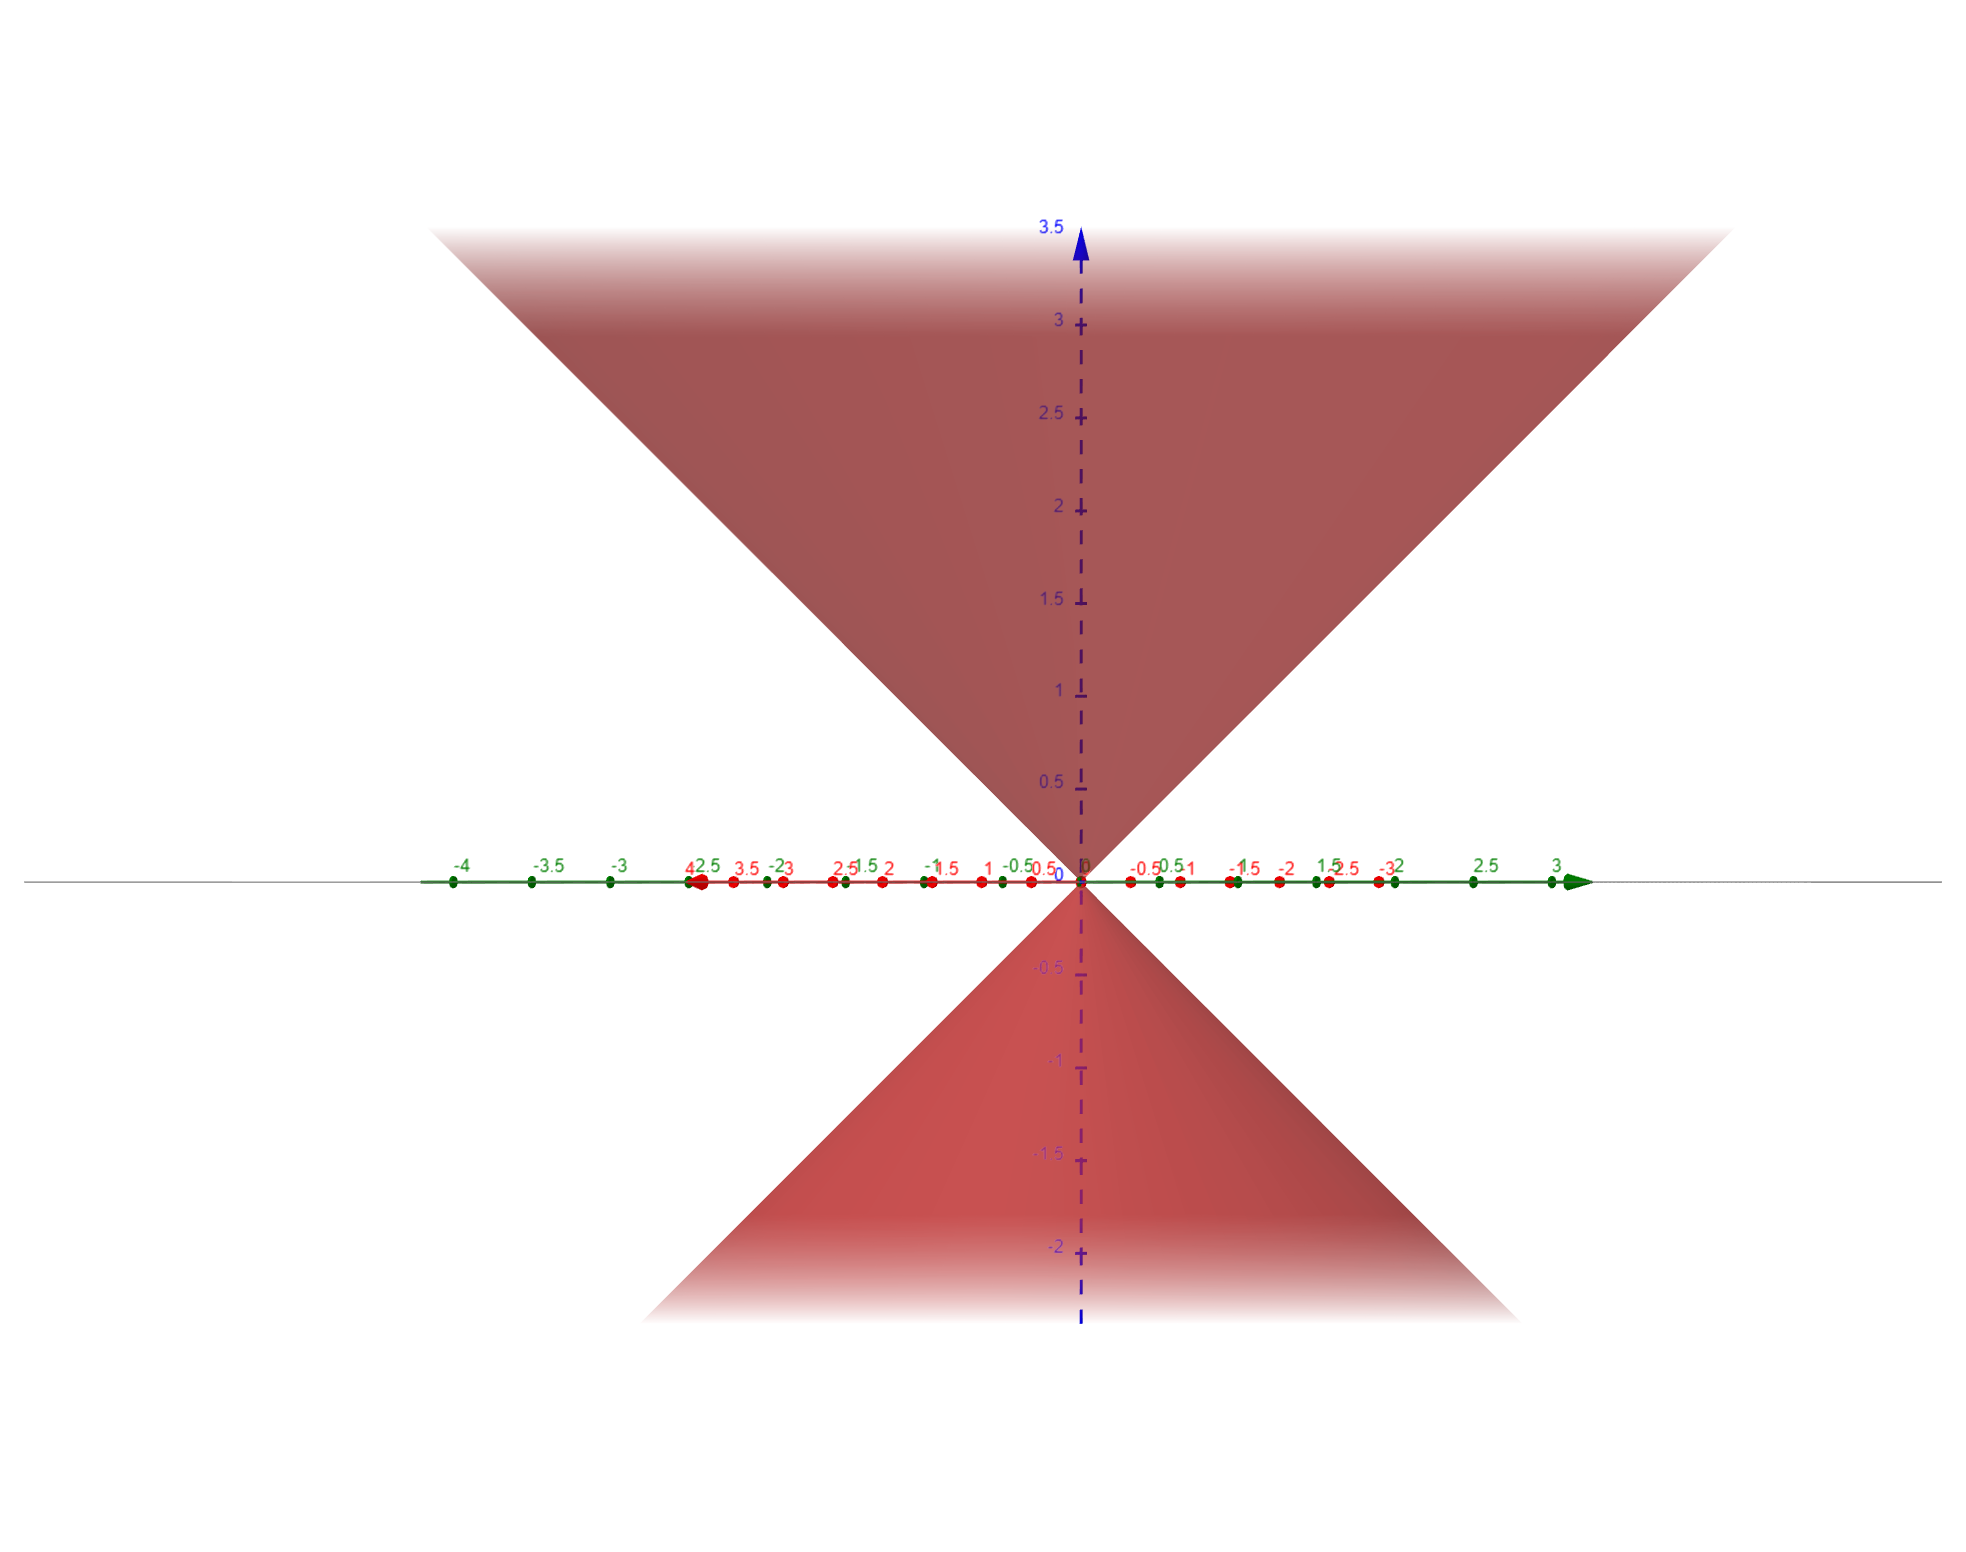
\includegraphics[width=.6\columnwidth]{cone_side.png}
            \caption{Side profile of a double cone.}
        \end{figure}
        If the angle of the vertex is to be $\pi/4$, then the slope of the line we see in the side profile for the $\rho z$-plane should make an angle with the $z$-axis of $\pi/8$. This happens when $C=2$, thus we take $\rho=2z$.
        
        \item If we give a curve in cylindrical coordinates, we want
        \[
        \curvegamma(t) = \begin{pmatrix} \rho(t) \\ \theta(t) \\ z(t) \end{pmatrix}.
        \]
        Since the radius is $1$, $\rho(t)=1$.  Pitch of 1 means that for every full revolution (i.e., $\theta$ increases by $2\pi$), we have $z$ increases by $1$. Thus $z=\frac{\theta}{2\pi}$.  Indeed, this means we are actually free to choose $\theta(t)$ as any increasing function (since we don't want to double back). The simplest is choosing $\theta=t$ and thus we arrive at $\rho(t)=1,~\theta(t)=t,~z(t)=\frac{t}{2\pi}$. 
    \end{enumerate}
    
        \item Recall that a hyperboloid of one sheet is given by
        \[
        x^2+y^2-z^2=C,
        \]
        where $C>0$.  Note that $\rho^2=x^2+y^2$, and thus
        \[
        \rho = \pm \sqrt{z^2+C}.
        \]
        
        One can also note that for $C=1$, $\frac{\rho}{z} = \tanh(t)$ for $t\in (-\infty,\infty)$ and $\theta \in [0,2\pi)$.  This gives the relationship $\rho(t)=\cosh(t)$ and $z(t)=\sinh(t)$ which is gives us the relationship between hyperbolic (co)sine and the trigonometric (co)sine. Namely, this hyperbola cross section is the \emph{unit} hyperbola and is closely related to the unit circle (see the simple shift in the sign of $z$ for the implicit equation). One could then take $C=-1$, to get the related two-sheeted hyperboloid.
\end{solution}

\end{document}